
%(BEGIN_QUESTION)
% Copyright 2006, Tony R. Kuphaldt, released under the Creative Commons Attribution License (v 1.0)
% This means you may do almost anything with this work of mine, so long as you give me proper credit

Studer følgende elektroniske nivåbryterkrets:

$$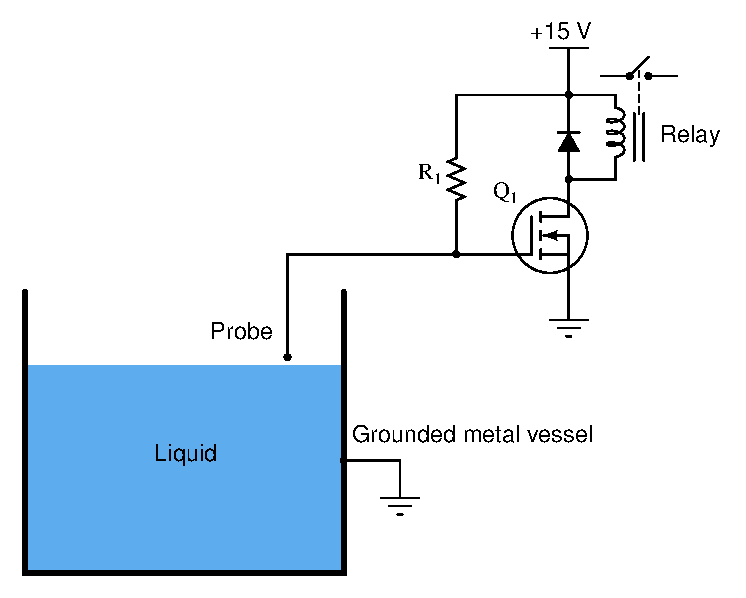
\includegraphics[width=15.5cm]{i00513x01.eps}$$

Identifiser hvilke typer prosessvæsker denne nivåbryteren kan brukes for, og hvorfor. Identifiser også hvilket ladderlogisk brytersymbol som passer for denne nivåbryteren:

$$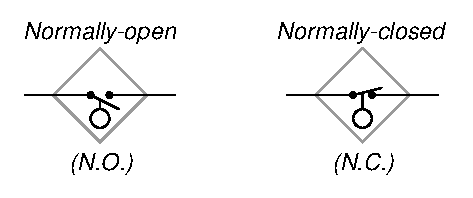
\includegraphics[width=15.5cm]{i00513x02.eps}$$

Bestem kvalitativt følgende spenningsfall i kretsen ved lavt nivå og høyt nivå (skriv ``lav'' eller ``høy'' spenning i stedet for å beregne eksakte verdier):

% No blank lines allowed between lines of an \halign structure!
% I use comments (%) instead, so that TeX doesn't choke.

$$\vbox{\offinterlineskip
\halign{\strut
\vrule \quad\hfil # \ \hfil & 
\vrule \quad\hfil # \ \hfil & 
\vrule \quad\hfil # \ \hfil \vrule \cr
\noalign{\hrule}
%
% First row
{\bf Komponent} & {\bf Lavnivå-tilstand} & {\bf Høynivå-tilstand} \cr
%
\noalign{\hrule}
%
% Another row
$R1$ &  &  \cr
%
\noalign{\hrule}
%
% Another row
$Q1$ (mellom drain og source) &  &  \cr
%
\noalign{\hrule}
%
% Another row
Reléspole &  &  \cr
%
\noalign{\hrule}
} % End of \halign 
}$$ % End of \vbox


\vfil 

\underbar{file i00513}
\eject
%(END_QUESTION)





%(BEGIN_ANSWER)

Dette er en vurderingsoppgave -- ingen svar eller hint oppgis!

%(END_ANSWER)





%(BEGIN_NOTES)

Et viktig forhold ved MOSFET-transistorer er at denne er en E-type (enhancement type) MOSFET, og derfor normalt av. Siden det er en {\it N-kanal} MOSFET, kreves et {\it positivt} gatesignal for å slå den på. Konkret må påtrykt gatespenning ha slik polaritet at gaten er mer positiv enn transistorens substrat. Da slår MOSFET-en inn og lar strøm gå gjennom reléspolen, slik at reléet energiseres og kontaktene lukker.

\vskip 10pt

En motstand mellom MOSFET-ens gate og +15 V-mateskinnen gir nødvendig bias for å slå transistoren på når ingen væske berører proben. Dette energiserer reléet og lukker bryterkontaktene, slik at kontaktene er lukket når proben er tørr. Dette er per definisjon en {\it normalt lukket} nivåbryter.

\vskip 10pt

Når væskenivået stiger høyt nok til å berøre proben, kortsluttes proben til jord. Da tvinges MOSFET-gaten til 0 volt, og MOSFET-en går tilbake til sin naturlige (av)tilstand. Reléet av-energiseres, og kontaktene åpner. Dermed gir høyt nivå åpne kontakter: akkurat oppførselen vi forventer av en {\bf normalt lukket} nivåbryter.

\vskip 10pt

Denne bryteren fungerer åpenbart bare med {\it ledende} væsker.

% No blank lines allowed between lines of an \halign structure!
% I use comments (%) instead, so that TeX doesn't choke.

$$\vbox{\offinterlineskip
\halign{\strut
\vrule \quad\hfil # \ \hfil & 
\vrule \quad\hfil # \ \hfil & 
\vrule \quad\hfil # \ \hfil \vrule \cr
\noalign{\hrule}
%
% First row
{\bf Komponent} & {\bf Lavnivå-tilstand} & {\bf Høynivå-tilstand} \cr
%
\noalign{\hrule}
%
% Another row
$R1$ & lav & høy \cr
%
\noalign{\hrule}
%
% Another row
$Q1$ (mellom drain og source) & lav & høy \cr
%
\noalign{\hrule}
%
% Another row
Reléspole & høy & lav \cr
%
\noalign{\hrule}
} % End of \halign 
}$$ % End of \vbox

\vskip 10pt

En interessant detalj i denne kretsen er {\it kommuteringsdioden} koblet parallelt med reléspolen. Legg merke til at orienteringen sikrer at dioden er av (ikke-ledende) mens reléspolen er energisert. Diodens eneste formål er å gi en ufarlig strømvei gjennom spolen når magnetfeltet kollapser (umiddelbart etter utkobling) og polariteten over spolen snur (spolen opptrer da som energikilde i stedet for last).

%INDEX% Switch, level: liquid conductivity

%(END_NOTES)

